\documentclass[12pt]{article}

\setlength{\parindent}{0em}
\setlength{\parskip}{.5em}

\usepackage{framed}
\newcounter{problem}
\newcounter{problempart}[problem]
\newcounter{solutionpart}[problem]
\newenvironment{problem}{\stepcounter{problem}\noindent{\bf\arabic{problem}.}}{\setcounter{problempart}{0}\setcounter{solutionpart}{0}}
\newenvironment{solution}{\par\textcolor{blue}\bgroup}{\egroup\par}
\newcommand{\qpart}{\stepcounter{problempart}${}$\\\noindent{(\alph{problempart})} }
\newcommand{\spart}{\stepcounter{solutionpart}${}$\\\noindent{(\alph{solutionpart})} }
\newcommand{\TODO}{\textcolor{red}{$\blacksquare$}}
\newcommand{\SOL}[1]{\textcolor{blue}{#1}}

\usepackage{hyperref}
\usepackage{fullpage}
\usepackage{amsmath,mathabx,MnSymbol}
\usepackage{color,tikz}
\usepackage{footnote,enumitem}
\usepackage{longtable}
\newcommand{\mx}[1]{\begin{pmatrix}#1\end{pmatrix}}
\newcommand{\mv}[1]{\begin{vmatrix}#1\end{vmatrix}}
\definecolor{dkgreen}{rgb}{0,.5,0}
\usepackage{algorithm}
\usepackage[noend]{algpseudocode}

\newcommand{\uu}{\mathbf{u}}
\newcommand{\bb}{\mathbf{b}}
\newcommand{\vv}{\mathbf{v}}
\newcommand{\cc}{\mathbf{c}}
\newcommand{\ww}{\mathbf{w}}
\newcommand{\xx}{\mathbf{x}}
\newcommand{\zz}{\mathbf{z}}
\newcommand{\ee}{\mathbf{e}}
\newcommand{\pp}{\mathbf{p}}
\newcommand{\qq}{\mathbf{q}}
\renewcommand{\AA}{\mathbf{A}}
\newcommand{\BB}{\mathbf{B}}
\newcommand{\MM}{\mathbf{M}}
\newcommand{\CC}{\mathbf{C}}
\newcommand{\DD}{\mathbf{D}}
\newcommand{\nn}{\mathbf{n}}
\newcommand{\gp}[1]{\left(#1\right)}
\newcommand{\half}{\frac{1}{2}}

\newcommand{\TODOL}[1]{\textcolor{red}{\underline{\hspace{#1 cm}}}}

\usepackage{listings}

\lstset{
  language=C++,
  showstringspaces=false,
  identifierstyle=\color{magenta},
  basicstyle=\color{magenta},
  keywordstyle=\color{blue},
  identifierstyle=\color{black},
  commentstyle=\color{green},
  stringstyle=\color{red}
}

\begin{document}

\title{CS130 - Barycentric coordinates}
\date{}
\author{Name: \TODOL7\qquad\qquad SID: \TODOL4}
\maketitle
\begin{center}
\end{center}

\begin{problem}
  In class, we formulated the barycentric coordinates through ratios of triangle areas.  We then implicitly assumed that $P = \alpha A + \beta B + \gamma C$. That is, the barycentric coordinates have the property that they interpolate the vertices of the triangle to the point $P$.  In this problem, you will prove this property.

  For the triangle $ABC$ illustrated, show that when the barycentric coordinates are determined through ratios of triangle areas, they interpolate the vertices to the point $P$.  That is, show that $P = \alpha A + \beta B + \gamma C$.

\begin{center}
  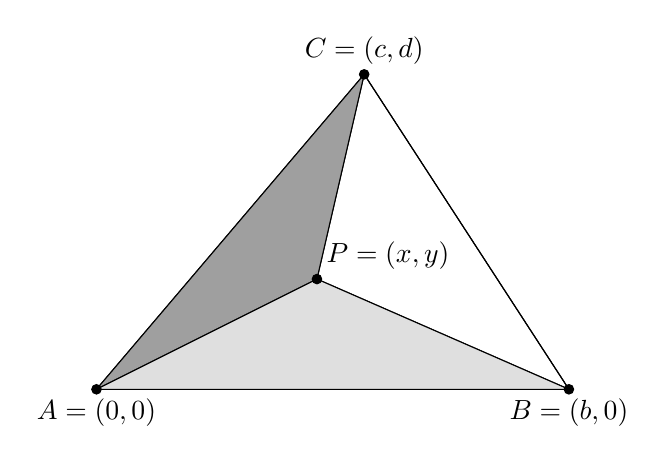
\begin{tikzpicture}[scale=2]
    \coordinate (A) at (0,0);
    \coordinate (A) at (0,0);
    \coordinate (B) at (3,0);
    \coordinate (C) at (1.7,2);
    \coordinate (P) at (1.4,.7);
    \draw (A) -- (B) -- (C) -- cycle;
    \draw (P) -- (B) -- (C) -- cycle;
    \draw[fill=gray!75] (A) -- (P) -- (C) -- cycle;
    \draw[fill=gray!25] (A) -- (B) -- (P) -- cycle;
    \draw[fill=black] (A) node[below]{$A = (0,0)$} circle (.03);
    \draw[fill=black] (B) node[below]{$B = (b,0)$} circle (.03);
    \draw[fill=black] (C) node[above]{$C = (c,d)$} circle (.03);
    \draw[fill=black] (P) node[above right]{$P = (x,y)$} circle (.03);
  \end{tikzpicture}
\end{center}
\end{problem}

\begin{solution}
  \textbf{\textcolor{red}{\TODO}}
\end{solution}


\begin{problem}
  The transformation $\xx \to \MM \xx + \bb$ is called an \textit{affine}
  transformation, where $\MM$ is a matrix and $\bb$ is a vector.  Let $P$ be a
  point inside triangle $ABC$.  The transformed point $P' = \MM P + \bb$ is
  inside the triangle with vertices $A' = \MM A + \bb$, $B' = \MM B + \bb$, and
  $C' = \MM C + \bb$.  Show that $P'$ has the same barycetric coordinates (in
  $A'B'C'$) as $P$ (in $ABC$).  That is, barycentric coordinates are preserved
  under affine transformations.
\end{problem}

\begin{solution}
  \textbf{\textcolor{red}{\TODO}}
\end{solution}

\begin{problem}
\begin{center}
  \begin{tikzpicture}[scale=2]
    \coordinate (A) at (0,.2);
    \coordinate (B) at (2.7,0);
    \coordinate (C) at (1.5,2);
    \coordinate (D) at (1.75,.7);
    \draw[fill=black] (A) node[below]{$A$} circle (.03);
    \draw[fill=black] (B) node[below]{$B$} circle (.03);
    \draw[fill=black] (C) node[above]{$C$} circle (.03);
    \draw[fill=black] (D) node[above right]{$D$} circle (.03);
    \draw[] (A) -- (B) -- (C) -- cycle;
    \draw[dashed] (D) -- (B);
    \draw[dashed] (D) -- (A);
    \draw[dashed] (D) -- (C);
  \end{tikzpicture}
\end{center}
How might one formulate barycentric coordinates for a tetrahedron?  Suggest formulas for computing them.
\end{problem}

\begin{solution}
  \textbf{\textcolor{red}{\TODO}}
\end{solution}

\end{document}

\item Barycentric coordinates
  \begin{itemize}
  \item 0,0,1 at vertices
  \item sum to 1
  \item nonnegative inside, inside-outside queries
  \item used for interpolation
  \item formulas for calculation from signed areas
  \end{itemize}
